% !TeX root = ../thuthesis-example.tex

\chapter{客户端数据预处理设计与实现\label{chap:client-design}}
本章介绍新 \emph{insertRecords} 写入机制中客户端侧对数据进行预处理的设计与实现。客户端对数据的预处理主要包括写入数据语义合法性校验、时间序列 ID 校验以及写入数据内存开销的计算。
\section{数据语义合法性校验设计}
在 \ref{sec:chap3-sec2} 节中,本文已经介绍过了目前 IoTDB 客户端对 \emph{insertRecords} 写入请求的处理流程,其主要负责的工作是对用户传入的参数进行语义合法性校验和时间序列数据和类型的序列化。在新的客户端设计中,对数据进行序列化和反序列化的过程将在 RPC 层统一进行,客户端无需再承担这一任务,但为了保证写入数据的正确性,对传入数据合法性校验的工作仍然需要保留。

\begin{figure}
  \centering
  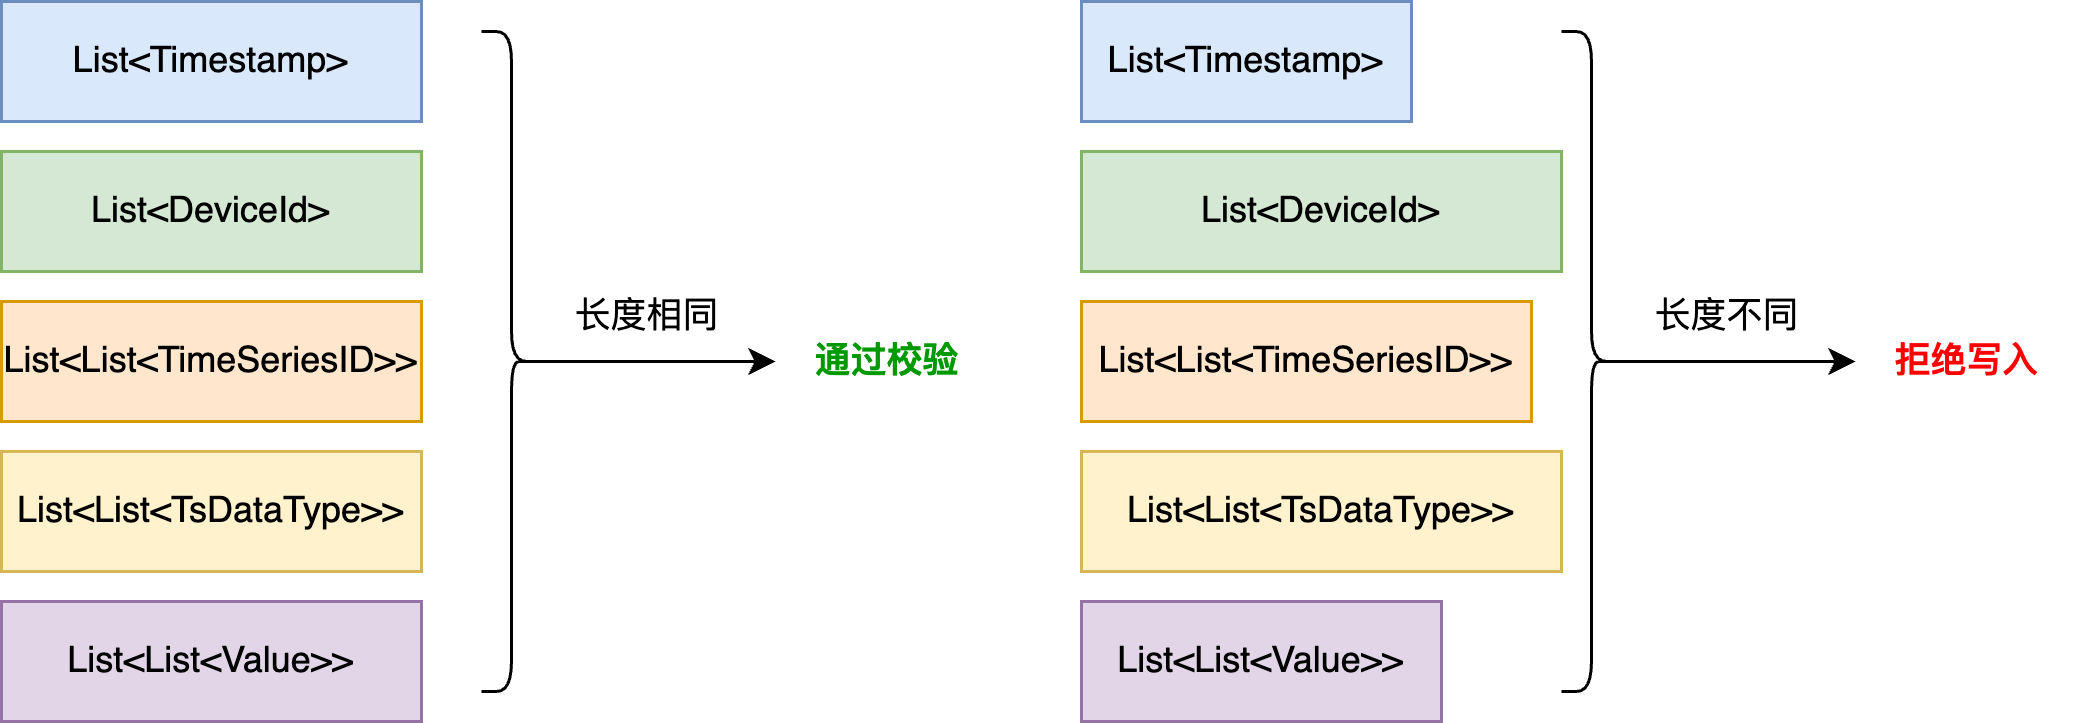
\includegraphics[width=\linewidth]{client-data-validate.png}
  \caption{写入数据语义合法性校验}
  \label{fig:client-data-validate}
\end{figure}

图 \ref{fig:client-data-validate} 展示了数据语义校验的两种情况。在合法的语义下,用户以列表为形式传入的参数之间的长度应该一致。如果出现了不一致的情况,客户端应该拒绝写入,并向上层应用抛出错误。由于传入的参数中还包含又嵌套列表,因此校验需要分两步进行,第一步校验第一层列表的长度是否相同,第二层再校验被嵌套的列表长度是否相同。伪代码如算法 \ref{alg:insert-records-validate} 所示。

\begin{algorithm}
  \caption{校验写入数据语义合法性}
  \label{alg:insert-records-validate}
  \small
  \begin{algorithmic}
    \REQUIRE deviceIds, timestamps, timeseriesIdsList, datatypesList, valuesList

    \IF{deviceIds.length $\neq$ timestamps.length \OR \\ timestamps.length $\neq$ timeseriesIdsList.length \OR \\ timeseriesIdsList.length $\neq$ datatypesList.length \OR \\ datatypesList.length $\neq$ valuesList.length}
     \STATE Reject insertion, and throw an exception
    \ENDIF

    \STATE $n \leftarrow \text{deviceIds.length}$
    \FOR{$i=1$ to $n$}
      \IF{timeseriesIdsList.at($i$).length $\neq$ datatypesList.at($i$).length \OR \\ datatypesList.at($i$).length $\neq$ valuesList.at($i$).length}
        \STATE Reject insertion, and throw an exception
      \ENDIF
    \ENDFOR

  \end{algorithmic}
\end{algorithm}

\section{时间序列 ID 校验设计}
IoTDB 中对时间序列 ID 的形式有一定的规定,参考最新的官方文档\footnote{https://iotdb.apache.org/zh/UserGuide/latest/Basic-Concept/Data-Model-and-Terminology.html},其中对时间序列 ID 的约束如下:
\begin{itemize}
  \item root 为系统保留字符,不可使用。
  \item 支持字母、数字、下划线以及 Unicode 中文字符。
  \item 对于包含特殊字符或者为实数的 ID,需要包含在反引号内。
\end{itemize}
时间序列 ID 校验的主要目的是检验用户输入的时间序列 ID 是否符合上述要求,如不符合,就会拒绝写入;如果符合,还会去除带有反引号的时间序列 ID 中的反引号,例如将 $`$\emph{123}$`$ 转换为 \emph{123}。检查时间序列 ID 是否合法的伪代码如算法 \ref{alg:validate-ts-id} 所示。
\begin{algorithm}
  \caption{时间序列 ID 校验}
  \label{alg:validate-ts-id}
  \small
  \begin{algorithmic}
    \REQUIRE timeseriesIdsList
    \ENSURE All id is valid
    \STATE let $n \leftarrow $timeseriesIdsList.length
    \STATE let $reserveWords$ be the set of reserve words in IoTDB
    \FOR{$i=1$ to $n$}
    \FOR{every $id$ in timeseriesIdsList.at($i$)}
    \IF{$id$ is surrounded by back quote}
      \STATE Remove $id$'s head and tail back quote. 
      \IF{All other back quotes appear in $id$ is in the form of $`$$`$.}
      \STATE Replace the origin $id$ with the one that head and tail back quote is removed.
      \ELSE
      \STATE Reject insertion and throw an exception.
      \ENDIF
    \ELSIF{$reserveWord$ contains $id$ \OR $id$ is a real number \OR $id$ does not match the timeseries id pattern}
    \STATE Reject insertion, throw an exception
    \ENDIF
    \ENDFOR
    \ENDFOR
  \end{algorithmic}
\end{algorithm}

\section{内存开销预计算设计}
IoTDB 中对一行数据进行内存管理时,会计算两类内存占用:数值占据的内存、时间序列元数据(ChunkMetadata)占用的内存。前者是时间序列数值和时间戳所占用的内存,后者是内存中为每条时间序列维护的统计信息,包括最大时间戳、最小时间戳、最大值、最小值、数据点个数等。

数值占据的内存主要由时间序列的类型决定,除文本类型的时间序列外,其他类型的时间序列同一序列下的每个数据点都占据了相同的内存大小。表 \ref{fig:data-type-mem-size} 显示了不同数据类型所占据的内存大小,其中文本类型是一个特殊的类型,其占用的内存大小由两部分组成:Java 中对 Text 对象的指针大小(8 字节)和文本中内容所占据的大小,所以文本类型的时间序列每一个数据点占用的内存可能都不一样,需要根据文本内容的长度计算。
\begin{table}
  \centering
  \caption{不同数据类型在占据内存的大小}
  \begin{tabular}{ll}
    \toprule
    数据类型 & 占据的内存大小 \\
    \midrule
    时间戳 & 8 字节 \\
    INT32 & 4 字节 \\
    INT64 & 8 字节 \\
    Float & 4 字节 \\
    Double & 8 字节\\
    Boolean & 1 字节 \\
    Text & 8 字节 + 文本的大小 \\
    \bottomrule
  \end{tabular}
  \label{fig:data-type-mem-size}
\end{table}

为了加速查询,IoTDB 会为每个写入内存表的时间序列维护一个元数据对象,其中记录了该条时间序列在内存表中数据的统计信息,包括该序列在内存表中数据的最小时间戳、最大时间戳、数据点个数、第一个插入的数据点和最后一个插入的数据点,如果是数值类型,还会记录最大值、最小值、数值总和。所以,一个元数据对象占用的内存空间和这个元数据对象描述的时间序列类型有关,表 \ref{fig:data-type-statistic-mem-size} 显示了不同数据类型的时间序列所对应的元数据对象占据的空间。

\begin{table}
  \centering
  \caption{不同数据类型的时间序列元数据对象在占据内存的大小}
  \begin{tabular}{ll}
    \toprule
    数据类型 & 占据的内存大小 \\
    \midrule
    INT32 & 157 字节 \\
    INT64 & 173 字节 \\
    Float & 157 字节 \\
    Double & 173 字节\\
    Boolean & 141 字节 \\
    Text & 173 字节 \\
    \bottomrule
  \end{tabular}
  \label{fig:data-type-statistic-mem-size}
\end{table}

在以上两种内存开销中,数值占用的内存开销的计算是与 IoTDB 的状态无关的,而时间序列元数据占用的内存计算则与 IoTDB 的状态有关。这是因为如果在写入数据时,如果内存表中已经包含了写入的时间序列的数据,那么就无需申请一块新的内存保存这条时间序列的元数据;反之,则需要申请新的内存,并且记录这块内存的大小。对于与 IoTDB 状态有关的内存开销计算是无法在客户端完成的,因为客户端并不清楚服务器的内存表中是否已经为待写入的序列创建了元数据对象。所以,客户端只计算数值项所占用的内存大小。

结合 \ref{sec:chap3-sec2} 节的介绍,一个 \emph{insertRecords} 写入请求中不同的行有可能会被定向到 IoTDB 中不同的数据分区。为了适应这一数据写入分配的模式,客户端在计算数值项的内存开销时也以一行数据为单位进行。对写入请求预计算数值项内存开销的过程如算法 \ref{alg:cal-mem-cost} 所示,计算的最终结果是一个整数数组,数组中的每一项都代表一行记录的数值项占用的内存大小。这一结果会通过 RPC 层一齐与待写入的数据发送给服务器,IoTDB 服务端在进行内存控制时只需计算元数据部分的内存开销即可,从而减轻了服务器的一部分计算负担。

\begin{algorithm}
  \caption{数值项内存开销计算}
  \label{alg:cal-mem-cost}
  \small
  \begin{algorithmic}
    \REQUIRE datatypesList, valuesList
    \STATE let $n \leftarrow$ datatypesList.length
    \STATE let $memCost$ be an integer array of size $n$
    \FOR{$i=1$ to $n$}
      \STATE let types $\leftarrow$ datatypesList.at($i$)
      \STATE let values $\leftarrow$ valuesList.at($i$)
      \STATE let $m \leftarrow$ types.length
      \STATE let $currCost \leftarrow 0$
      \FOR{$j=1$ to $m$}
        \STATE Add memory cost to $currCost$ according to types.get($j$)
        \IF{types.get($j$) is Text}
          \STATE Calulate the memory cost of values.get($j$) according to its length, and add it to $currCost$
        \ENDIF
      \ENDFOR
      \STATE $memCost[i] \leftarrow currCost$
    \ENDFOR
    \RETURN $memCost$
  \end{algorithmic}
\end{algorithm}

\section{客户端请求格式转换}
从 \ref{sec:chap3-sec3-1} 节的实验中,我们发现了当一个写入请求中,一个设备有多行数据时,\emph{insertRecords} 的写入性能不如 \emph{insertTablets} 的写入性能。从系统的设计与实现出发分析这一现象的原因,是因为 \emph{insertTablets} 接口将一个设备的数据都集中在了一起,而 \emph{insertRecords} 将同一个设备的数据分散在了不同的行中,并且这些行记录了一些重复的信息。\emph{insertTablets} 把一个设备所有请求数据都集中在了一起,并且

\section{客户端数据预处理实现}
前文中已经介绍了在客户端进行写入语义校验、时间序列 ID 校验和内存开销预计算的设计与算法,本节中将介绍在客户端侧对这些流程的实现。IoTDB 目前有 Java、C++、Python、Rust 等客户端,其中被使用最广泛的是 Java 语言客户端,因此本文中对客户端的改进工作都基于 Java 语言客户端进行。

对写入数据的语义合法性校验是客户端处理所有数据的第一步,因为对具有非法语义的数据进行任何处理都是没有意义的。本步骤较为简单,本质上就是对比多个 List 结构体的长度是否一致,在实现时通过两个嵌套的 for 循环就可以完成,本文不再赘述。

\begin{figure}
  \centering
  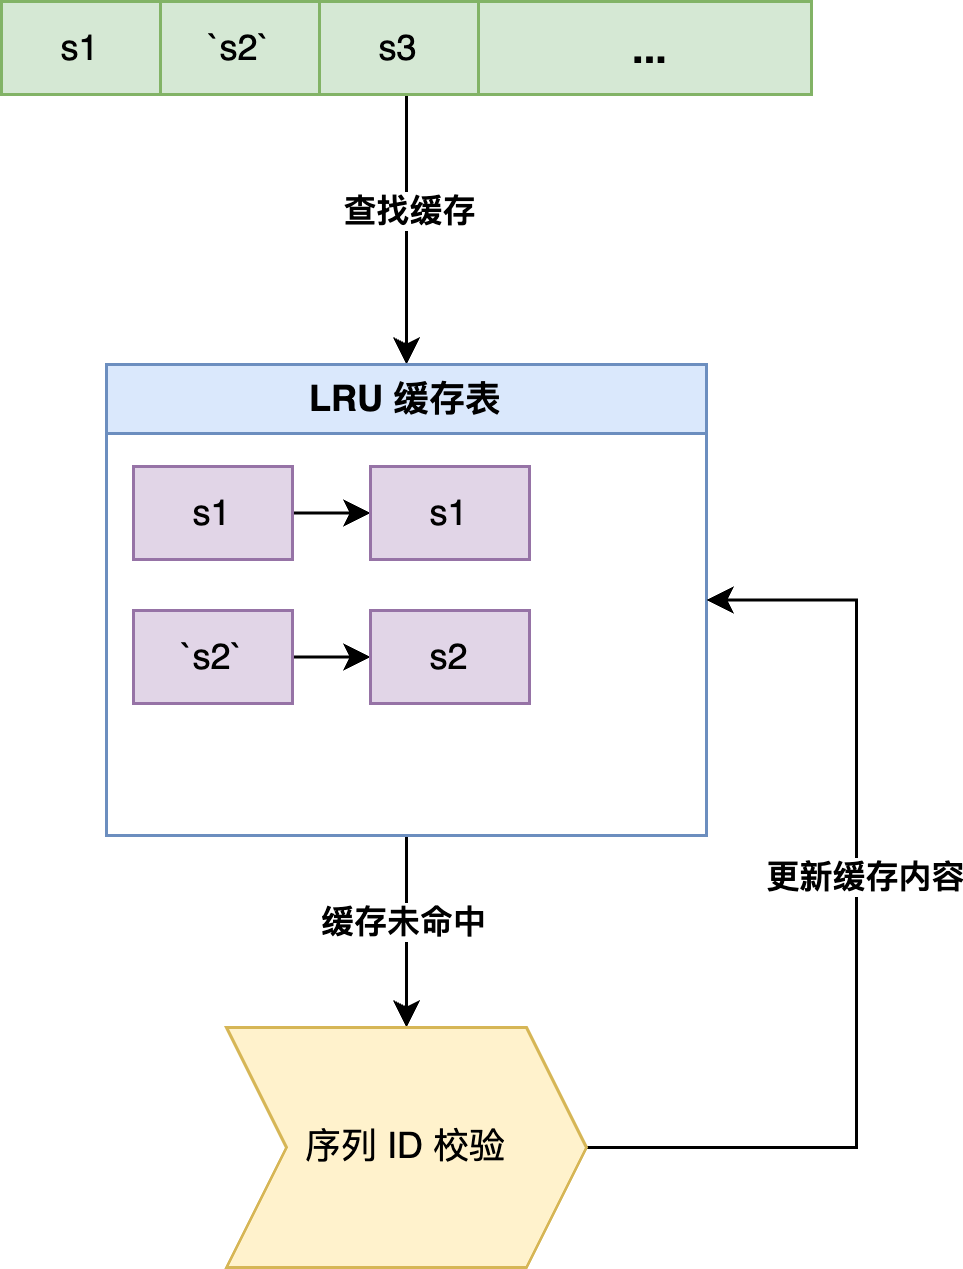
\includegraphics[width=0.7\linewidth]{lru-ts-id-validate.png}
  \caption{带有 LRU 缓存的时间序列 ID 检验过程}
  \label{fig:lru-ts-id-validate}
\end{figure}

在算法 \ref{alg:validate-ts-id} 描述的对时间序列 ID 校验的过程中,对传入的每一个时间序列 ID 都要进行一次检查。这样的实现并不是最高效的,因为通过 \emph{insertRecords} 接口传入的数据中,可能存在一个设备下的多行数据,不同行数据之间包含相同的时间序列 ID;即使是不同设备之间的时间序列 ID 也可能存在相同的情况。例如在车联网场景下有几万个设备,但是每个设备几乎都包含相同的时间序列 ID,因为这些 ID 对应的是车辆上同一种型号的传感器。 如图 \ref{fig:lru-ts-id-validate} 所示,为了充分利用序列 ID 的这一特点,在实现时笔者加入了一个哈希表结构作为缓存,将一个时间序列 ID 映射到一个字符串,这个字符串代表经过脱反引号处理后得到的时间序列 ID。在对每一个序列 ID 检查前,都先检查这个哈希表中是否已经缓存了该时间序列 ID 的校验结果,如果有则可以跳过检查,如果没有则进行检查,并将检查得到的脱引号后的结果保存在该哈希表中。为了避免一次写入请求中包含的不同的时间序列 ID 数量过多,缓存哈希表中的项数过多导致客户端内存不足,该哈希表通过最近最少使用策略(Least Recently Used,LRU)策略管理缓存项,当缓存项的数目超过一定阈值,就会及时清除那些最近未被使用的项,以节约内存空间。

\begin{figure}
  \centering
  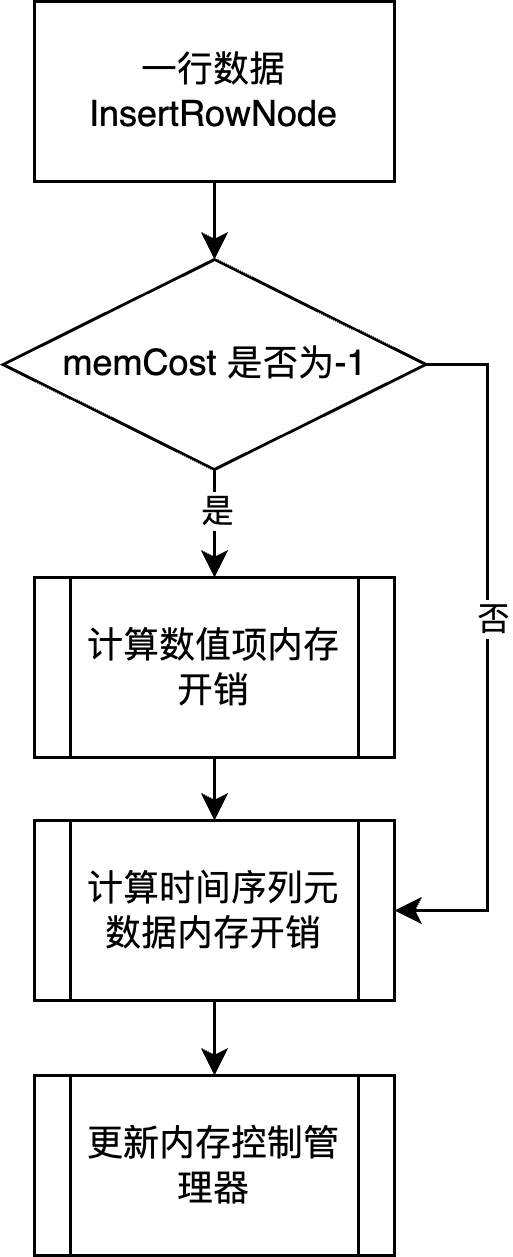
\includegraphics[width=0.25\linewidth]{mem-control.png}
  \caption{存储引擎兼容新旧客户端进行内存控制的流程}
  \label{fig:mem-control-compatibility}
\end{figure}


内存开销预计算的实现不仅要在客户端侧实现,也要在存储引擎侧配合实现。这主要是因为内存控制是在存储引擎侧进行的,客户端计算了数值项内存开销之后存储引擎理论上就无需计算了。但是,由于升级客户端往往需要重启写入程序,而写入程序通常和上层的业务程序部署在同一个进程中,所以用户在升级存储引擎后,往往不能及时升级客户端,而是需要等待业务侧合适的时机才能进行。因此,存储引擎不仅需要适配新客户端,也要对原有的客户端保持兼容。


客户端按照算法 \ref{alg:cal-mem-cost} 对每一行数据计算出数值项内存开销后,将其一起通过 RPC 层传输到服务器。存储引擎在对一行数据进行写入时,这一行数据以 InsertRowNode 结构体表示。笔者在 InsertRowNode 中增加一个新的字段 \emph{memCost},代表该行数据的数值项所占据的内存。在接收到客户端计算的数值项内存开销的结果后,IoTDB 会将这些结果记录到每一行数据对应的 InsertRowNode 的 \emph{memCost} 字段中。在处理没有计算数值项内存开销的客户端传输的请求时,则把 InsertRowNode 的 \emph{memCost} 字段设置为 -1,代表该数值未被计算。如图 \ref{fig:mem-control-compatibility} 所示,存储引擎在处理 InsertRowNode 的写入时,通过判断 \emph{memCost} 字段是否为 -1 来辨识是否已经通过客户端预计算了数值项的内存大小。如果已经计算过,那么存储引擎只需要计算时间序列元数据的内存开销;如果没有计算过,那么存储引擎则需要计算数值项和时间序列元数据的内存开销。

\section{本章小结}
本章介绍了在客户端侧进行数据预处理的若干步骤设计,包括写入数据的语义合法性校验、时间序列 ID 校验和写入数据的数值项内存开销计算,并且介绍了在实现时为了性能和兼容性而进行的优化方法。